\chapter{Experiments}
There are 8 experiments in this thesis which can be classified into four parts: basic models, mixed data model, fine-tuning models, and increment fine-tuning models. In the first part, I train models in order to compare with other experiments and choose some parameters. In mixed-data part, I try to train models using both source and target data. When it comes to fine-tuning part, I use target data to fine-tune source model. Finally, I try to add target data gradually into fine-tuned model.

\section{Cross Validation}
I use cross validation to validate my model and divide training/validation/testing sets. Cross validation is validation techniques for assessing how the results of a model will generalize to an independent dataset and estimating how accurately a predictive model will perform in practice. I divide dataset into 10 subsets. Then I choose one to be testing set while the rest part is training set and validation set. For the rest 9 subset, I choose 10 \% to be validation set and the rest 90 \% is training set. The two tables below shows how we divide training/validation/testing sets for source data and target data.


\begin{figure}[H]
    \hfil
    \begin{minipage}[t]{0.9\textwidth}
        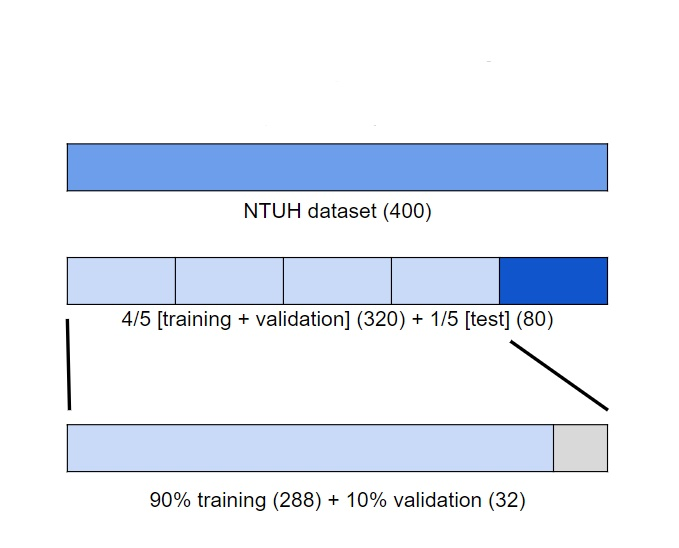
\includegraphics[width=\textwidth]{fig/cross.png}
        \caption{\label{fig:parallel1} AUC for mixed Source Data and Target Data}
    \end{minipage}
    \hfil
\end{figure}
 
 \begin{table}[H]
\centering
\caption{training/validation/testing set (10 folder)}
\begin{tabular}{|l|l|l|l|l|} 
\hline
~            & source H & source T & target H (tcia) & target T (msd)  \\ 
\hline
train        & 330      & 382      & -               & -               \\ 
\hline
validation   & 37       & 42       & -               & -               \\ 
\hline
source test  & 41       & 47       & 0               & 0               \\ 
\hline
target test~ & 0        & 0        & 8               & 18              \\
\hline
\end{tabular}
\end{table}
\begin{table}[H]
\centering 
\caption{training/validation/testing set (B) (10 folder)}
\begin{tabular}{|l|l|l|l|l|} 
\hline
amount of data   & tar H (train) & tar T (train) & tar H (val) & tar T (val)  \\ 
\hline
40       & 11      & 25      & 1               & 3               \\ 
\hline
80 & 22       & 50       & 2               & 6               \\ 
\hline
120 & 34       & 74       & 4               & 8               \\ 
\hline
160 & 45        & 99        & 5               & 11              \\
\hline
200 & 56       & 125       & 6               & 14               \\ 
\hline
\end{tabular}
\end{table}
 ~\\
\section{Basic Models}
In this part, I train models in order to compare with other experiments and choose parameters for other experiments.
\subsection{Train Models Using Only Source Data (B1)}
First, I want to calculate the prediction results if the model is only consider about source data. The results will compare with other experiment results to see how much other methods will improve. The amount of target data fixes 0.
\subsection{Train Models Using Only Target Data (B2)}
I want to calculate the prediction results if the model is only consider about target data. I want to know if how much data is needed to get a sufficiently nice model. The amount of target data varies from 40 to 200.
\subsection{Choose the Number of Fixed Layers in Fine-tuning Experiments (B3)}
All experiments in this thesis use a simplified VGG model for training, however it's better to fix some layers since the target dataset is small for fine-tuning. The goal of this experiment is to find the number of fixed layers in fine-tuning experiments. The amount of target data fixes 200.
~\\
\section{Mixed Data Models}
\subsection{Mixed Data Models (M1)}
In this part, we mixed source and target data to train model. The amount of target data varies from 40 to 200 while the amount of source data fixed.
~\\
\section{Fine-Tuning Models}
\subsection{Fine-Tuning Models (F1)}
In this part, I fine-tuned the model trained in (B1) using target data. I fixed the first three layers in this experiments and use target data to modify the rest layers. The amount of target data varies from 40 to 200.
~\\
\section{Increment Fine-Tuning Models}
Suppose we get an unlabeled target dataset, we want to first label some data that best improve the model performance and use them to fine-tune model. If the AUC performance is not good enough, we need to repeat all steps and fine-tune model using another selected dataset.

\subsection{AIFT Selection Method}
AIFT selection method is applied in increment learning. It calculate the entropy and diversity of the patch-based prediction result of each patient data, and select the data that has the maximum entropy and diversity. For each unlabeled patient data, first I split it into patch-based data. Then use the model generated by source data to predict each patch and get a list of prediction results. Secondly, if the mean value of the list is higher than 0.5, choose the top quarter of list. Otherwise choose the last quarter of list. Then calculate the entropy and diversity of the prediction list. Finally choose a set of patient data that has the highest entropy and diversity and label them. 

\subsection{Fine-tuning Using Selected/Random Target Data (S1/R1)}
This experiment is applied to observe the AUC performance and validate if the selection method AIFT works compared to random selection. We replace the select method to random selection to valid that the selection method really works. 

\subsection{Fine-tuning Using Different Amount of Target data (S2/R2)}
We gradually add selected subset of target data until all target data is used to observe the AUC performance. The amount of target data varies from 40 to 200.

\subsection{Fine-tuning Using Selected/Random Target Data with 66 epochs (S3/R3)}
This experiment is the same as S1/R1 except the number of epochs. I reduce the number of epochs so that the calculation cost is the same as basic fine-tuning method. 